\section{PROPOSED FRAMEWORK}
\label{sec:framework}
In the proposed framework, aging tolerance is achieved by specifically assigning useful/beneficial skews into the designs, based on timing borrowing. The beneficial skews are progressively created by different aging behaviors of clock paths, due to the different duty cycles of clock signal caused by DCCs. Moreover, high-$V_{th}$ assignment for clock buffers is also incorporated in the proposed framework to explore more beneficial skews, further improving the aging tolerance of designs.
The overall flow of the proposed framework is depicted in Figure~\ref{fig:flow}, where we focus the following three issues:
\begin{enumerate}[leftmargin=*]
	\item \textbf{Minimization of clock period:} The clock period can be minimized since the performance degradation of the logic circuit is \enquote{tolerated} as a result of useful clock skews. The minimum required clock period thus implies maximum level of aging tolerance. As depicted in Figure~\ref{fig:flow}, a binary search for optimal clock period is involved in the proposed framework.
	\item \textbf{DCC deployment:} The problem of  DCC deployment is formulated as a Boolean Satisfiability (SAT) problem. Therefore, the key of our framework is to represent the problem in \textit{conjunctive normal form} (CNF). A CNF representation is a conjunction of one or more clauses, where each clause is a disjunction of one or more Boolean variables. Thanks to the efficiency of existing SAT solvers, the solution can be obtained efficiently. The end result of this formulation is the locations (in the existing clock tree) of DCCs, such that the required clock period of the given circuit under $n$-year BTI is minimized when aging-induced clock skews are considered. 
	\item \textbf{High-$V_{th}$ assignment for clock buffers:} The problem of high-$V_{th}$ assignment for clock buffers is also formulated as a SAT-based problem, represented in CNF and solved by existing SAT solvers.
\end{enumerate}

\begin{figure}
	%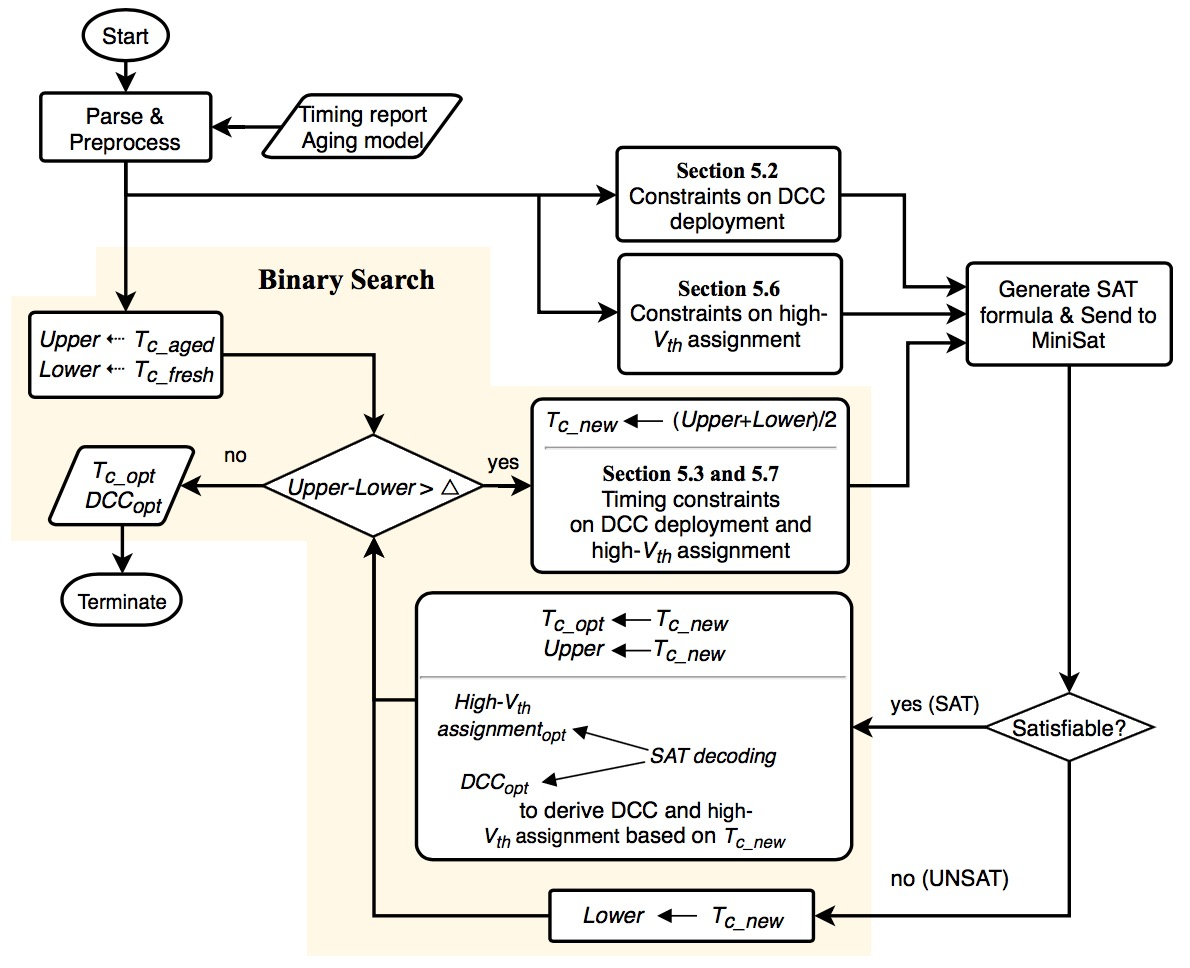
\includegraphics[width=1\columnwidth]{Flow_chart.png} %IEEE Journal
	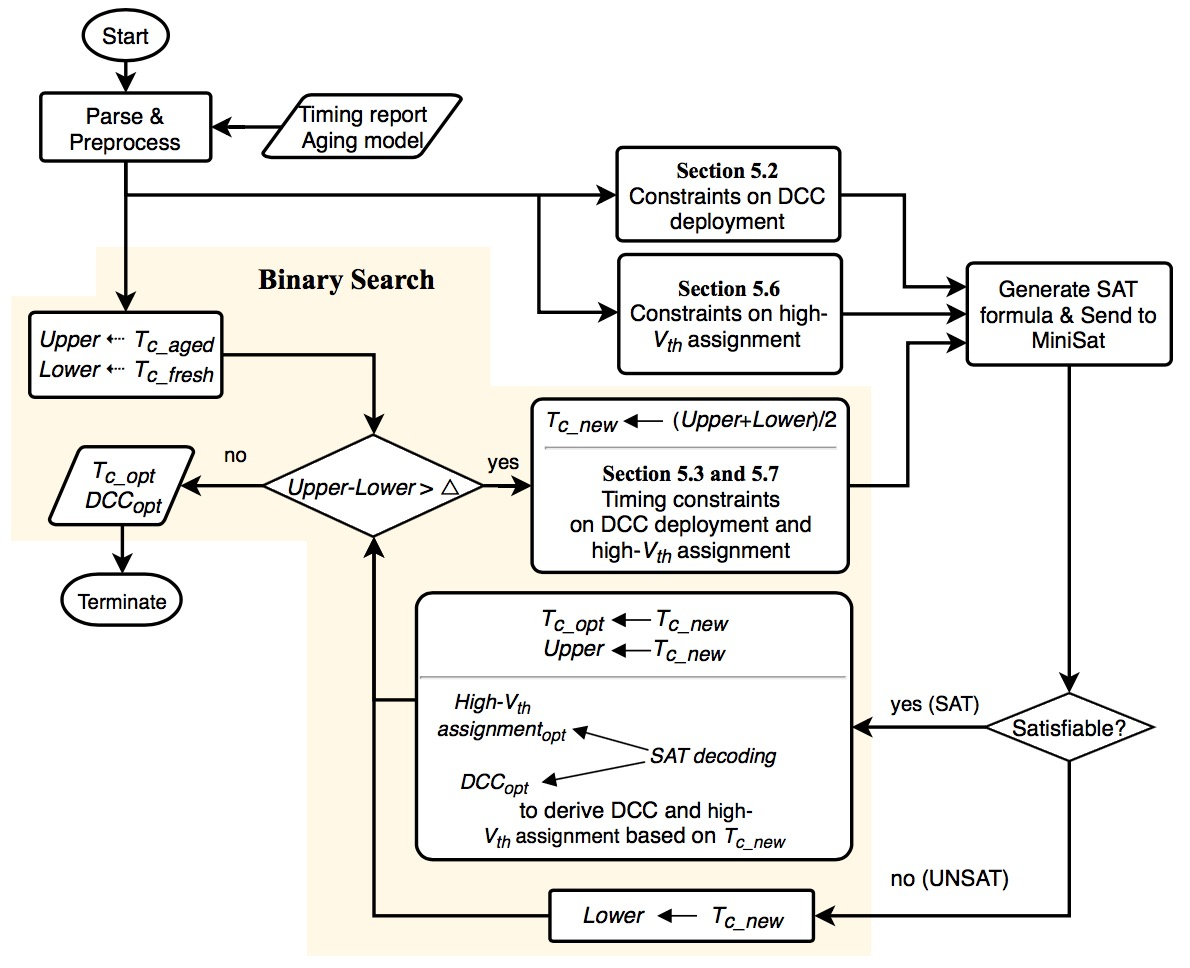
\includegraphics[width=0.85\columnwidth]{Flow_chart.png} %ACM Journal
	\caption{The overall flow of MAUI}
	\label{fig:flow}
\end{figure}
 

The section is organized as follows: Section~\ref{subsec:eddcd} explains how the proposed problem of DCC deployment/insertions are encoded with Boolean variables. Section~\ref{subsec:dccccc} and Section~\ref{subsec:tccc} describe three major components, DCC constraints and timing constraints, for our SAT-based formulation and how they are translated into legal SAT formula, i.e., CNF representation. Finally, Sections~\ref{sec:VTA}-\ref{sec:VTA:timing} introduce the additive improvements by high-$V_{th}$ assignment for buffers.

\afterpage{ 
\begin{figure}
	\centering
	%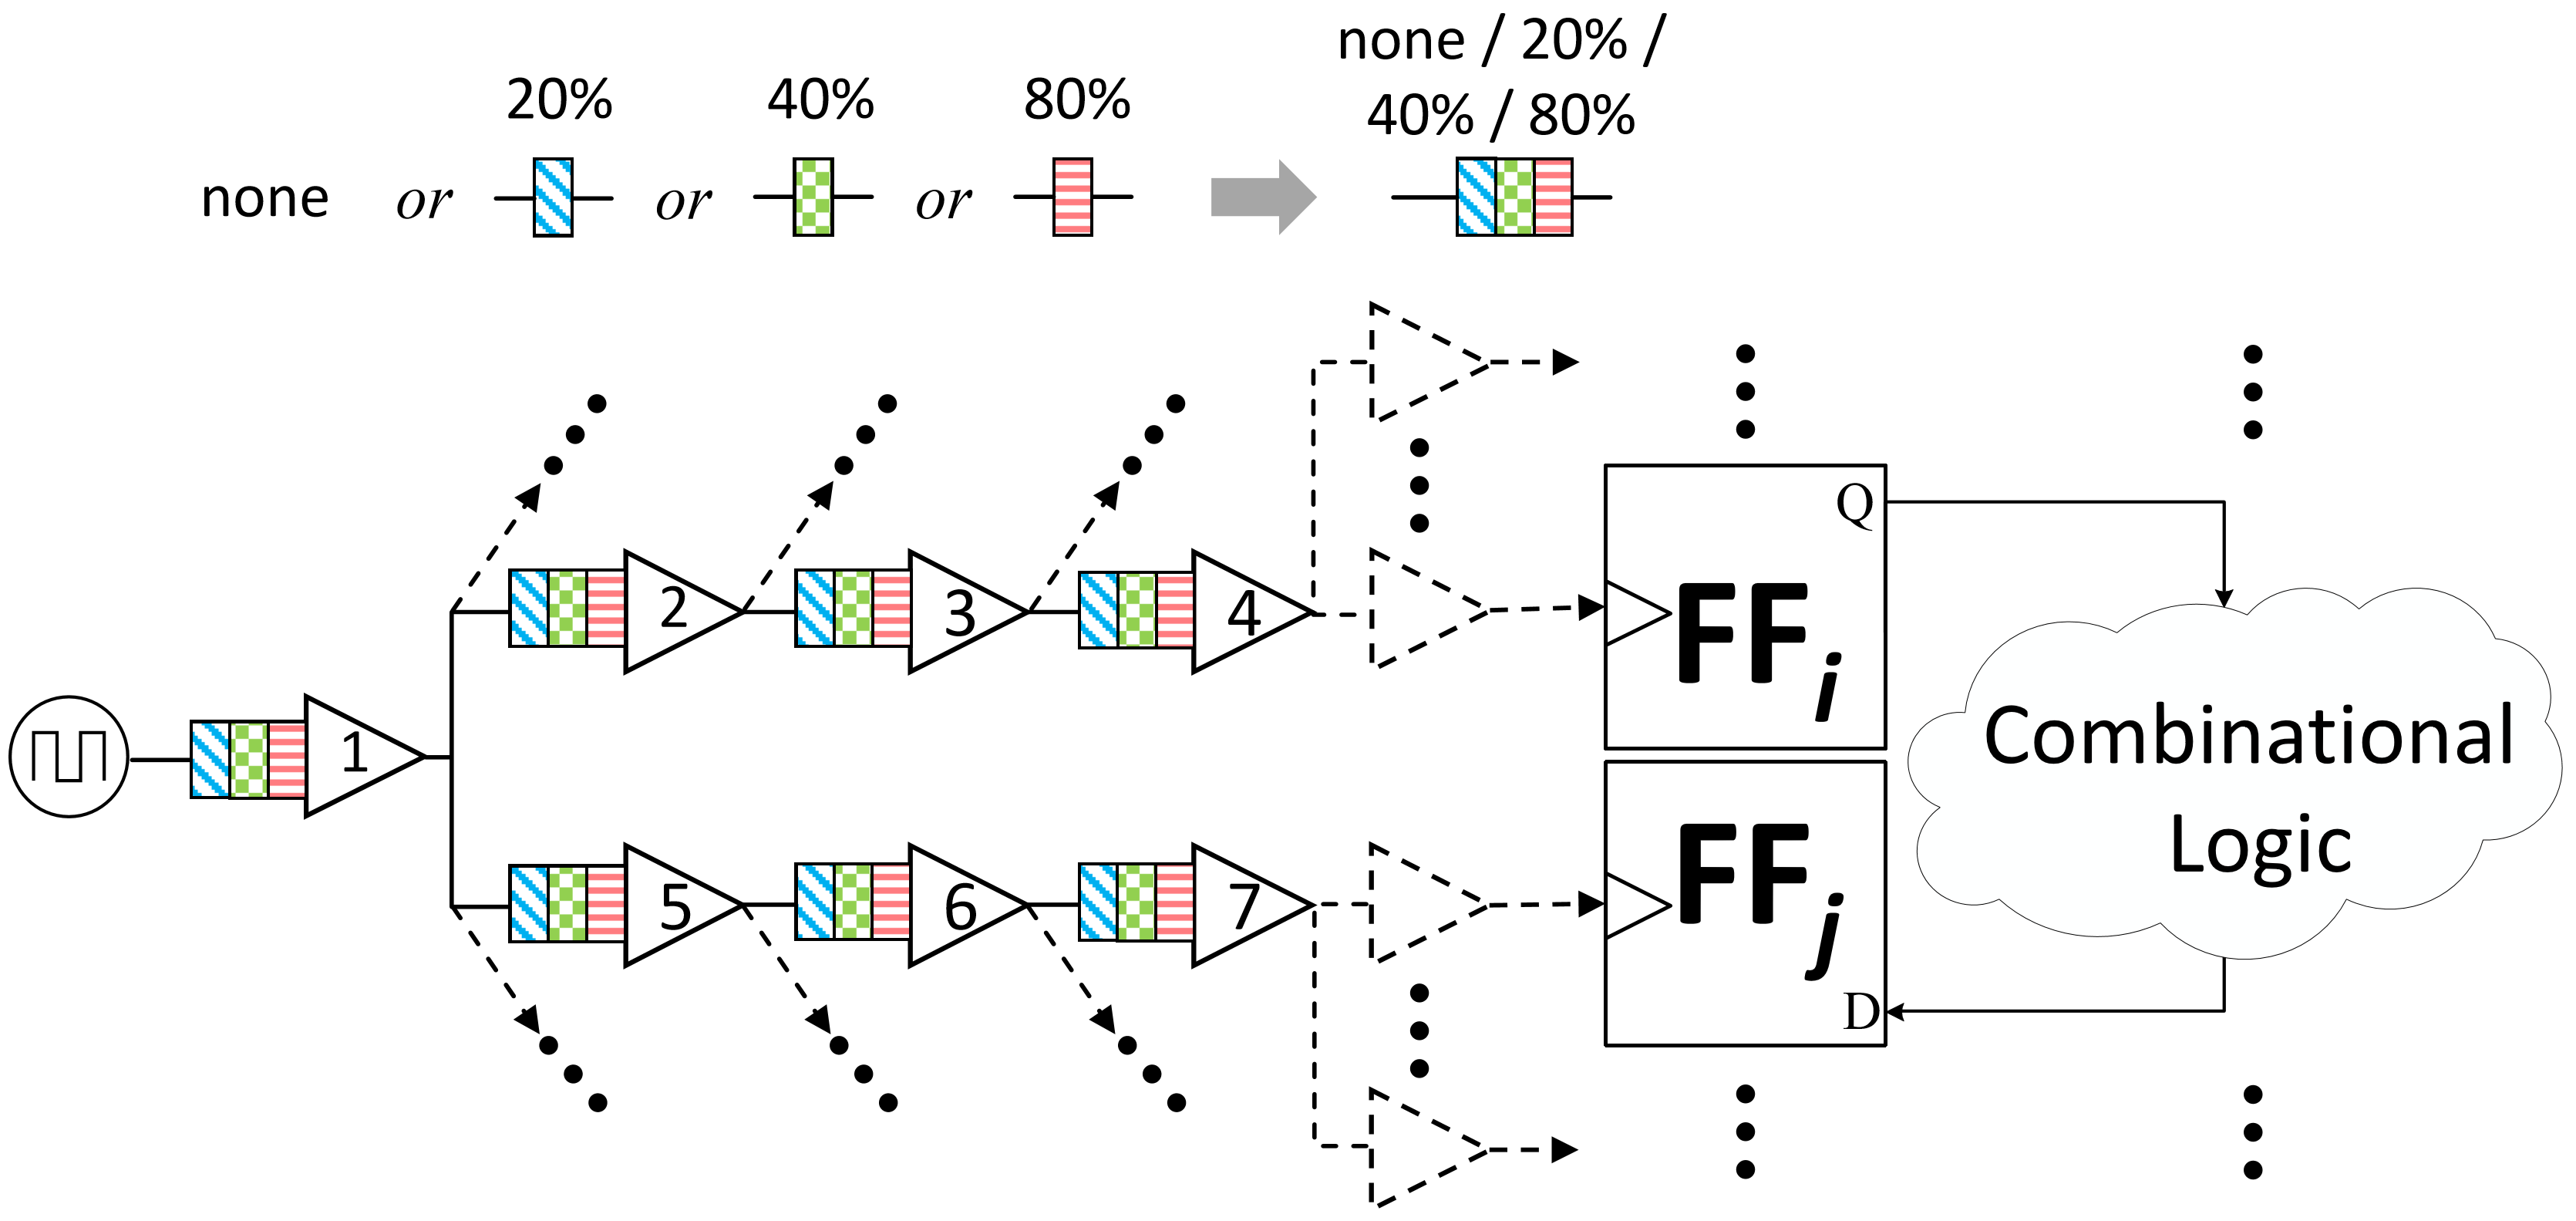
\includegraphics[width=1.0\columnwidth]{All_types_of_DCCs.png} %IEEE Journal
	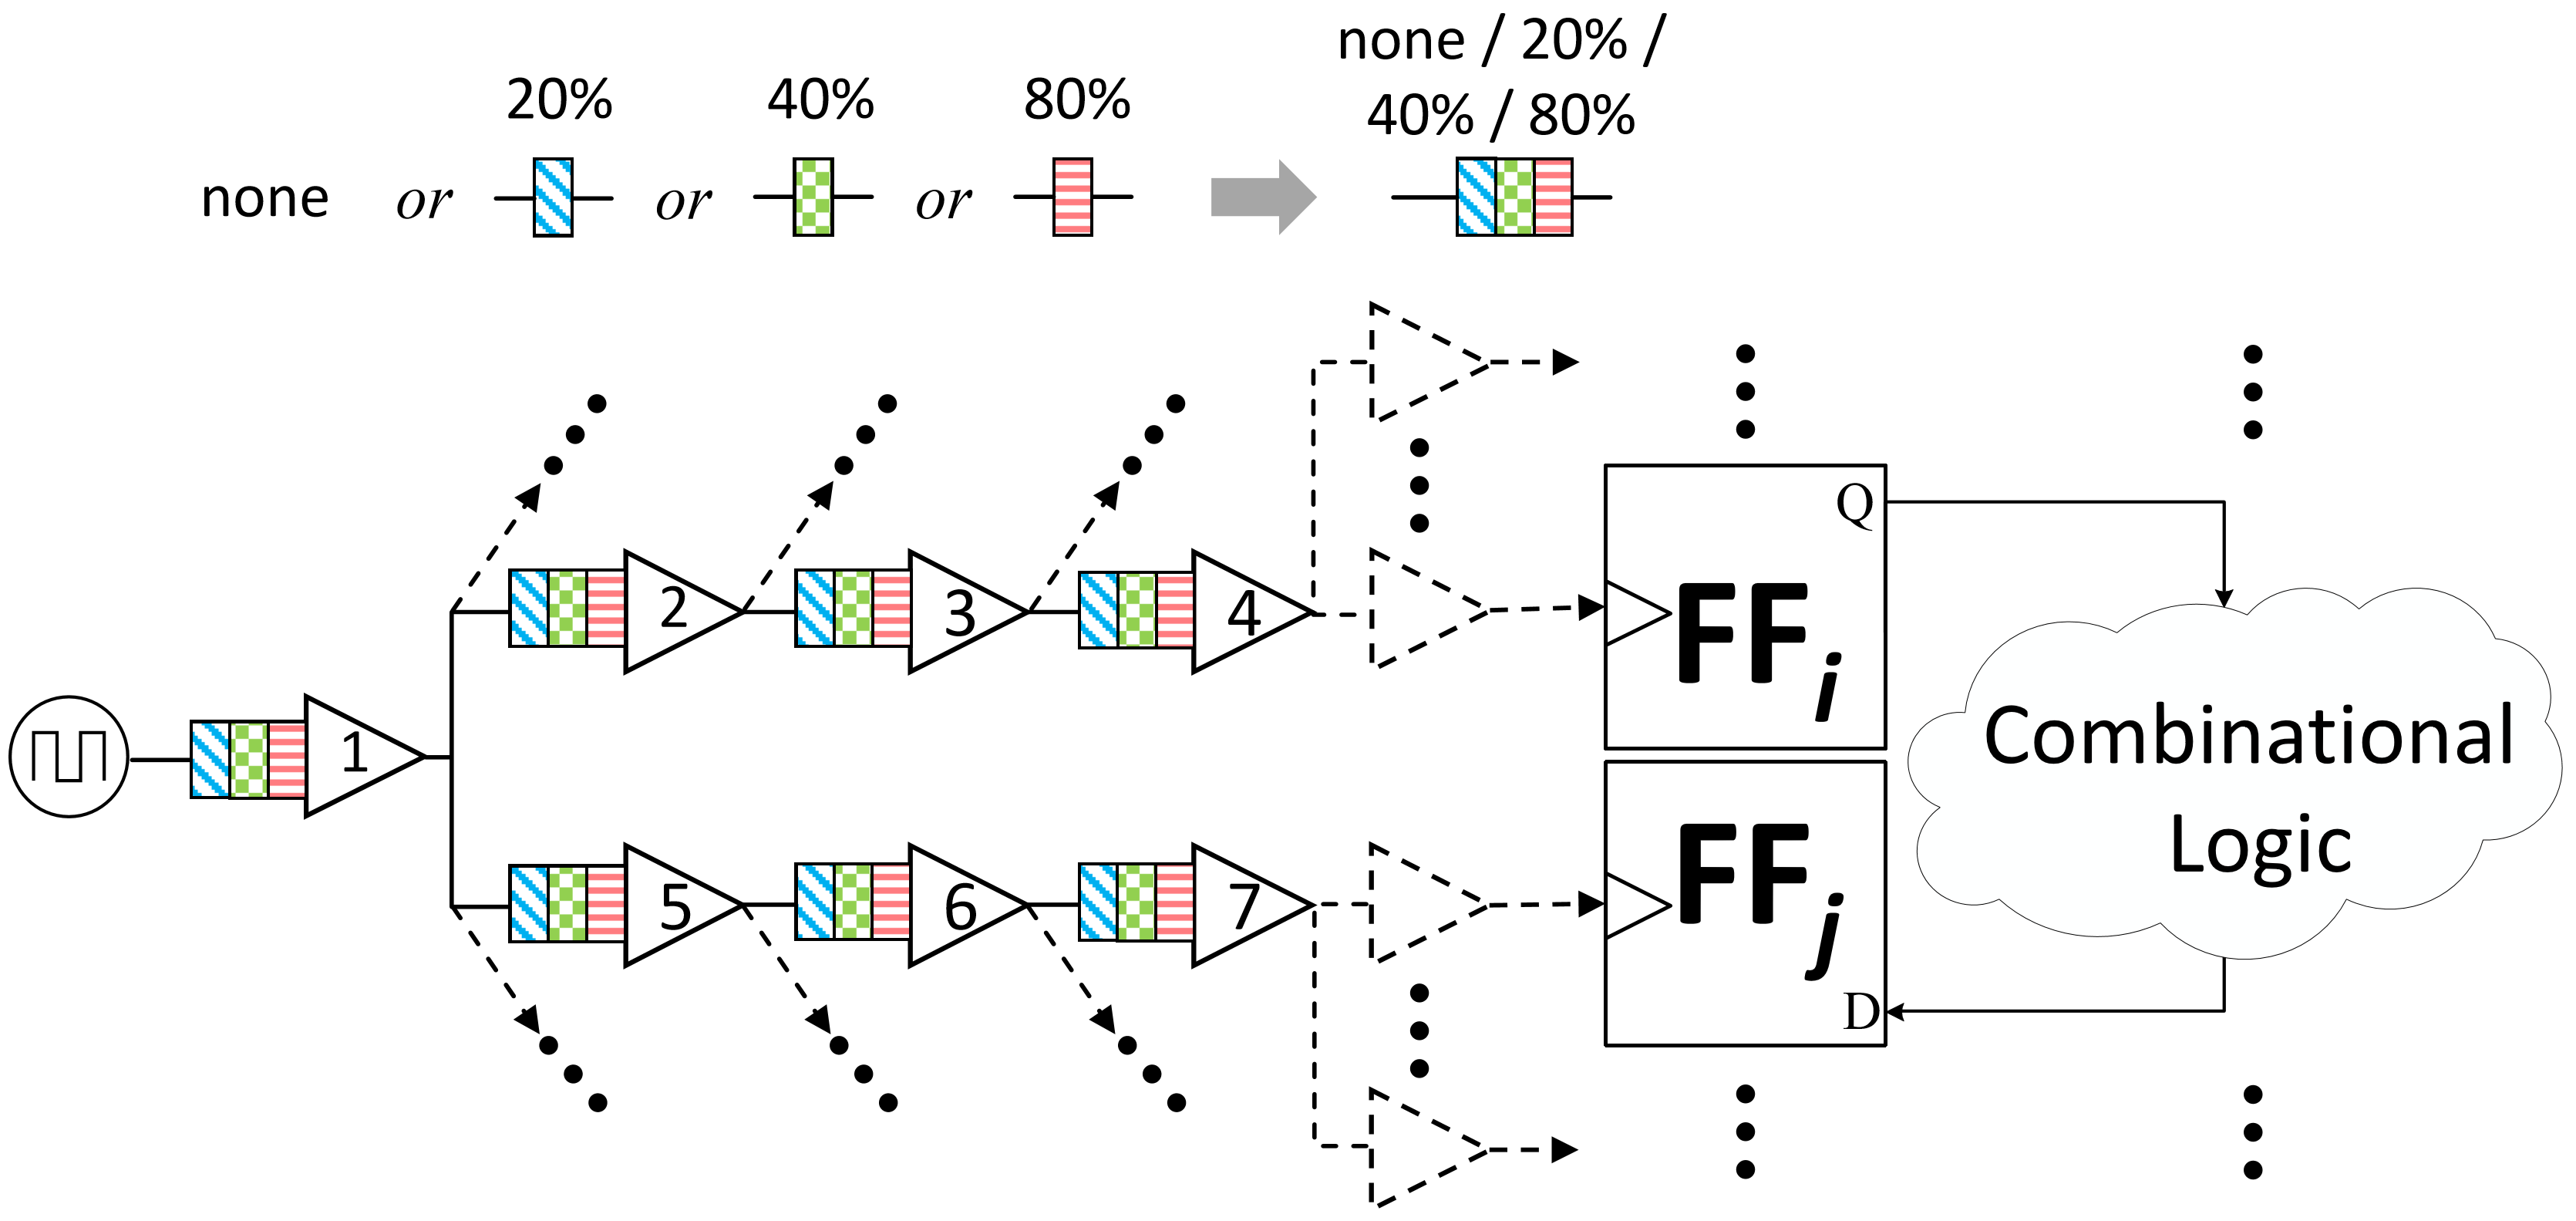
\includegraphics[width=0.7\columnwidth]{All_types_of_DCCs.png} %ACM Journal
	\caption{Generalized DCC insertion for a target pair of flip-flops} 
	\label{fig:dcctype} 
\end{figure}
}

%(3) DATE 2018
\subsection{Boolean Encoding for DCC Deployment}
\label{subsec:eddcd}
The problem of DCC deployment needs to be encoded into Boolean representation before being transformed into a SAT-based formulation. Assume that a total of $N$ types of DCCs can be chosen. Including the DCC-free case where no DCC is inserted, there are ($N$ + 1) possibilities of DCC insertion for each clock buffer. We denote a clock buffer by $p\left(1 \leq p \leq P\right)$ where $P$ is the total count of clock buffers and $p$ is buffer index. For each clock buffer, there exist two types of Boolean variables, {\fontsize{9}{10}$B_{p,q}$} ($1 \leq q \leq Q $, $Q = \lceil \lg (N + 1)\rceil$), where {\fontsize{9}{10}$\left\{B_{p,1}, B_{p,2},\dotsc, B_{p,Q}\right\}$} encode the aforementioned ($N$ + 1) possibilities of DCC insertion at the input of buffer $p$.



Without loss of generality, we assume $N$ = 3. Thus, there are three types of DCCs, assumed to be 20\%, 40\%, and 80\% DCCs, as shown in Figure~\ref{fig:dcctype}. Therefore, three Boolean variables are used for encoding four possibilities of DCC at any buffer. The four possibilities can be encoded as follows:

\begin{comment}
{\small
\begin{tabular}{  c  c  c  c  }
  	 & Leader type & DCC type & $\{B_{p,3}, B_{p,2}, B_{p,1}\}$ \\ 
  	(1)\quad & Nominal $V_{th}$ ($V_{th}^n$) & None & \{0, 0, 0\} \\ 
  	(2)\quad & $V_{th}^n$ &20\% &  \{0, 0, 1\} \\ 
  	(3)\quad & $V_{th}^n$ &40\% &  \{0, 1, 0\} \\ 
  	(4)\quad & $V_{th}^n$ &80\% &  \{0, 1, 1\} \\ 
	(5)\quad & high-$V_{th}$ ($V_{th}^h$) & None & \{1, 0, 0\} \\ 
  	(6)\quad & $V_{th}^h$ & 20\% &  \{1, 0, 1\} \\ 
  	(7)\quad & $V_{th}^h$ & 40\% &  \{1, 1, 0\} \\ 
  	(8)\quad & $V_{th}^h$ & 80\% &  \{1, 1, 1\} \\ 
\end{tabular}}
\end{comment}
%(5) DATE 2018
{\small
\begin{tabular}{ c c c }
\centering
   & DCC type & $\left\{B_{p,2},B_{p,1}\right\}$ \\
  (1)\quad & None & \{0, 0\} \\
  (2)\quad & 20\% &  \{0, 1\} \\
  (3)\quad & 40\% &  \{1, 0\} \\
  (4)\quad & 80\% &  \{1, 1\} \\
\end{tabular}}
\afterpage{
\begin{figure*}
    \centering
    \subfigure[Class 2-1: one DCC on the common clock path (e.g., at buffer 1)]{
    	\label{fig:sub:dcci1}
        %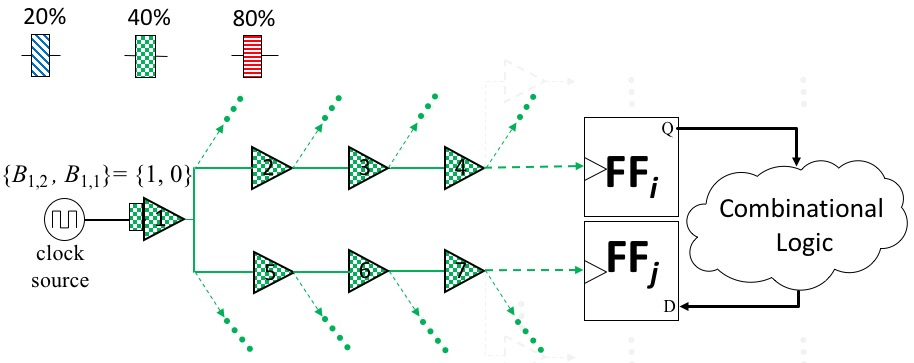
\includegraphics[width=0.92\columnwidth]{A_examlpe_of_DCC_placement1.png}  %IEEE Journal
        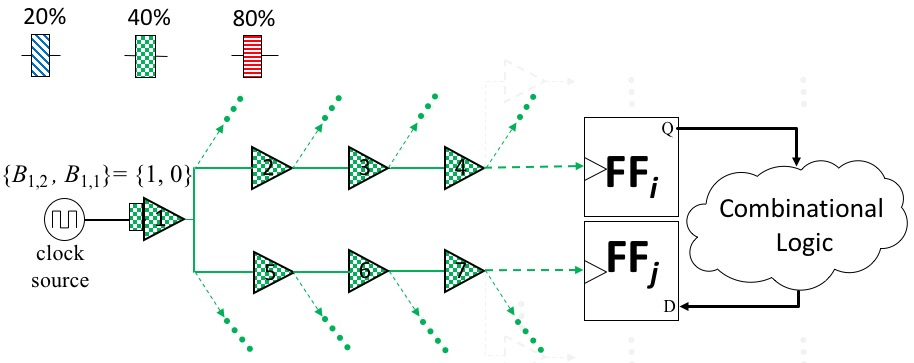
\includegraphics[width=0.65\columnwidth]{A_examlpe_of_DCC_placement1.png}  %ACM Journal
    }
    \hspace{1cm}
    \subfigure[Class 2-2: one DCC on one of the divergent clock paths, or class 3: two DCCs, one on each of the divergent clock paths]{
    	\label{fig:sub:dcci2}
        %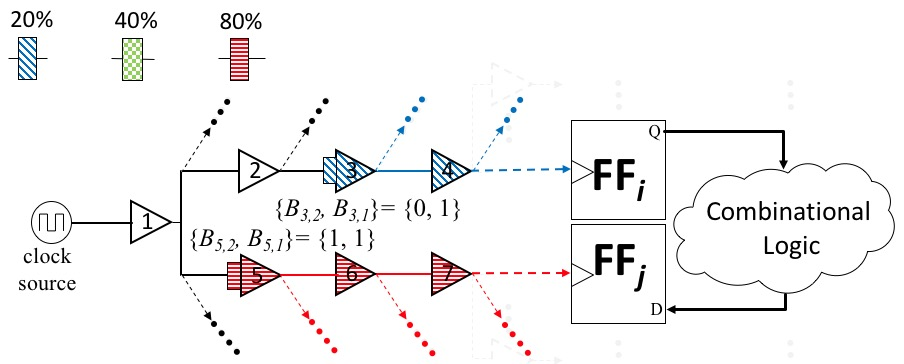
\includegraphics[width=0.92\columnwidth]{A_examlpe_of_DCC_placement2.png}  %IEEE Journal
        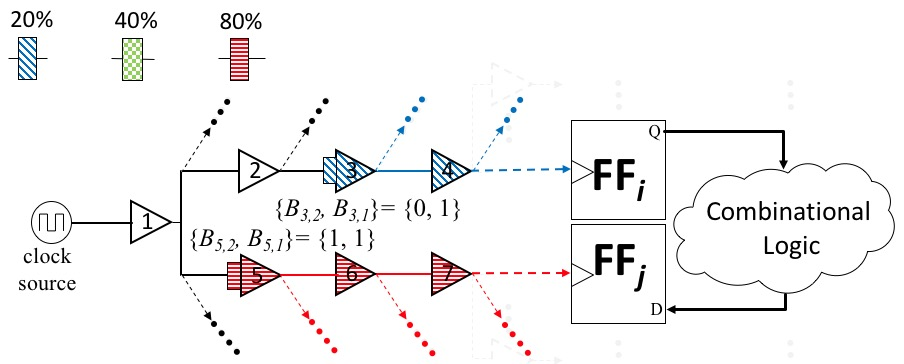
\includegraphics[width=0.65\columnwidth]{A_examlpe_of_DCC_placement2.png}  %ACM Journal
    }
    \caption{Examples of DCC insertion}
    \label{fig:dccinsert}
\end{figure*}
}

For example, in Figure~\ref{fig:sub:dcci2}, a 20\% DCC and an 80\% DCC are inserted at buffer 3 and buffer 5, respectively. Therefore, {\fontsize{9}{10}{$\left\{B_{3,2}, B_{3,1}\right\}$ = \{0, 1\}}}, {\fontsize{9}{10}{$\left\{B_{5,2}, B_{5,1}\right\}$ = \{1, 1\}}}, and {\fontsize{9}{10}{$\left\{B_{p,2}, B_{p,1}\right\}$ = \{0, 0\}}} for $p$ = 1, 2, 4 , 6 or 7.

The 20\% DCC will mitigate the aging of buffer 3 and its downstream buffers, while the 80\% DCC will aggravate the aging of buffer 5 and its downstream buffers. It can be found that, if a DCC is deployed deep in the clock tree (i.e., close to the flip-flops), the count of affected buffers is limited and thus the overall impact of aging mitigation/aggravation on $C_i$/$C_j$ may be insignificant, diminishing the benefit from deploying DCCs for aging tolerance.  To avoid the phenomena, we set a rule of prohibiting DCC deployment at a clock tree level larger/deeper than a specified boundary. This rule also greatly reduces the complexity of our SAT-based formulation because a significant fraction of buffers are excluded from being considered inserted DCC at their inputs. For example, in Figure~\ref{fig:dcctype}, those dashed buffers and their downstream buffers are excluded. 

%(2) B
\subsection{Constraints on DCC Deployment}
\label{subsec:dccccc}

Figure~\ref{fig:dcctype} shows a generalized example of DCC insertion for a pair of flip-flops (\ce{FF_i} and \ce{FF_j}) where there exist aging-critical paths from \ce{FF_i} to \ce{FF_j}. A path is defined as an aging-critical path if, in the presence of aging, it is possible to determine the clock period of the circuit. Every pair of flip-flops between which there exist aging-critical paths needs to be considered and here, we use this generalized example to illustrate our SAT-based formulation.

In Figure~\ref{fig:dcctype}, buffers 1 - 7 are candidate locations for DCC insertions and according to the encoding scheme explained in Section~\ref{subsec:eddcd}, two Boolean variables are introduced for each of the seven buffers to encode four possibilities of DCC insertions. Considering all seven buffers, there are a total of 16,384 (= $4^7$) possibilities for DCC insertions, just for this pair of flip-flops. This makes the SAT-based formulation intractable due to the explosion of clause count. Therefore, we set up the following constraints on DCC insertion: 

{\noindent \textbf{\uline{DCC constraint: At most one DCC on a single clock path (from the clock source to one of the flip-flops)}}}

In order to ensure no more than one DCC on any clock path, we can use the Boolean variables introduced for DCC insertion, i.e., {\fontsize{9}{10}$B_{p,q} \left(1 \leq p \leq P, 1 \leq q \leq Q = \lceil \lg (N + 1) \rceil \right)$}, to generate some clauses which suppress the occurrence of having two DCCs on a clock path. Consider buffer 2 (encoded by {\fontsize{9}{10}$\left\{B_{2,2}, B_{2,1}\right\}$}) and buffer 3 (encoded by {\fontsize{9}{10}$\left\{B_{3,2}, B_{3,1}\right\}$}) in Figure~\ref{fig:dcctype}. If there is a DCC at buffer 2 (i.e., {\fontsize{9}{10}$\{B_{2,2}, B_{2,1}\} \not\equiv \{0, 0\}$}), then there must no DCC at buffer 3 (i.e., {\fontsize{9}{10}$\{B_{3,2}, B_{3,1}\} \equiv \{0, 0\}$}), and vice versa. The constraint can be formally written as:
{\fontsize{9}{10}
\begin{gather*}
\left(\{B_{2,2}, B_{2,1}\} \equiv \{0, 0\}\right) \lor \left(\{B_{3,2}, B_{3,1}\} \equiv \{0, 0\}\right)
\end{gather*}}
Next, it can be translated into 4 CNF clauses:
{\fontsize{9}{10}
\begin{equation*}
\begin{split}
(\neg B_{2,1}\lor\neg B_{3,1}) \land (\neg B_{2,1}\lor\neg B_{3,2}) \land (\neg B_{2,2}\lor\neg B_{3,1}) \land (\neg B_{2,2}\lor\neg B_{3,2})
\end{split}
\end{equation*}}
Any pair of buffers along a single clock path should be constrained in this way. Among buffers 1- 7 in Figure~\ref{fig:dcctype}, there are 12 pairs: $\langle1, 2\rangle$, $\langle1, 3\rangle$, $\langle1, 4\rangle$, $\langle1, 5\rangle$, $\langle1, 6\rangle$, $\langle1, 7\rangle$, $\langle2, 3\rangle$, $\langle2, 4\rangle$, $\langle3, 4\rangle$, $\langle5, 6\rangle$, $\langle5, 7\rangle$, $\langle6, 7\rangle$. Each pair translates to 4 clauses and a total of 48 clauses will be generated accordingly.

With DCC constraints and corresponding clauses, we can drastically reduce the possibilities of DCC insertions to be formulated. In the above example where the 48 clauses associated with DCC constraints are generated, the possibility count of DCC insertions drops from 16,384 to 103. In the next subsection, we describe what the 103 possibilities are and how they are translated into the final CNF representation.

%(3) C
\subsection{Timing Constraints}
\label{subsec:tccc}
Given a pair of flip-flops, if there exists one logic path between them, the timing (i.e. setup-time and hold-time) constraints must be met based on the inequalities~(\ref{eq:tsu}) and~(\ref{eq:th}). Different types of DCCs reveal different influence on clock latency. Consider the lifespan specification of 10 years in Figure~\ref{fig:sub:dcci2}: the delay of each clock buffer is changed after 10 years. The clock latency of \ce{FF_i} (i.e., $C_i$) is the sum of clock buffer delays from clock source to \ce{FF_i}: 
\begin{gather*}
C_i = \tau_1 + \tau_2 + \tau_3 + \tau_4 +\dotsb \\
C_j = \tau_1 + \tau_5 + \tau_6 + \tau_7 +\dotsb
\end{gather*}
where $\tau_k$ is the delay of buffer $k$. Consider aging effects on $C_i$ and $C_j$: 
\begin{gather*}
C_{i\_aged} = 1.13 \times \left(\tau_1 + \tau_2\right) + 1.09 \times \left(\tau_3 + \tau_4 + \dotsb\right)\\
C_{j\_aged} = 1.13 \times \tau_1+ 1.16 \times \left( \tau_5 + \tau_6 + \tau_7 + \dotsb \right)
\end{gather*}
where $C_{i\_aged}$ and $C_{j\_aged}$ denote aged $C_i$ and $C_j$, respectively. Next, we apply Equations~(\ref{eq:tsu}) and~(\ref{eq:th}) to check whether timing constraints will be violated under this DCC deployment.

\noindent \textbf{\uline{Timing constraint: No existence of timing violation}}

Given one clock period $T_c$ derived by binary search, one aging-critical path, and its associated clock network, all possible DCC deployments can be classified into 3 classes according to the number of DCCs used. Furthermore, due to the aforementioned DCC constraints, the SAT solver will only output a DCC deployment where there does not exist more than one DCC along any clock path. Thus, in the following discussion, the deployment with more than one DCC along a single clock path can be ignored. In each class, if the DCC deployment causes a timing violation within 10 years (i.e., the lifespan specification), then the deployment will be transformed into CNF clauses, such that the solver will not output the deployment as results. Here, we explain the generation of CNF clauses by using the example in Figure~\ref{fig:dccinsert}.\\

\noindent \textbf{Class 1:} No DCC is inserted on either clock path

Consider the situation that no DCC is inserted at buffers 1- 7. If it causes a timing violation along the aging-critical path within 10 years, then the Boolean representation of the deployment,
{\fontsize{9}{10}
\begin{gather*}
\left(\{B_{1,2}, B_{1,1}\} \equiv \{0, 0\} \right) \land \left( \{B_{2,2}, B_{2,1}\} \equiv \{0, 0\} \right) \land \dotsb 
\land \left( \{B_{7,2}, B_{7,1}\} \equiv \{0, 0\} \right),
\end{gather*}}
equivalent to the following CNF clause:
{\fontsize{9}{10}
\begin{gather*}
\left(B_{1,2} \lor B_{1,1} \lor B_{2,2} \lor B_{2,1} \lor \dotsb \lor B_{7,2} \lor B_{7,1} \right),
\end{gather*}}
should be generated such that the solver will not output the corresponding deployment in the result if the CNF is satisfiable. In this case, a total of 1 CNF clause is generated.\\

\noindent \textbf{Class 2:} Inserting one DCC

This class can be further classified into 2 sub-classes based on the location of inserted DCCs. \\
\textit{Class 2-1:} Inserting one DCC on the common clock path

In Figure~\ref{fig:dccinsert}, buffer 1 is on the common clock path. Consider the DCC insertion shown in Figure~\ref{fig:sub:dcci1}: if the insertion of a 40\% DCC at buffer 1 causes a timing violation within 10 years, then the Boolean representation of the DCC deployment,
{\fontsize{9}{10}
\begin{gather*}
\left(\{B_{1,2}, B_{1,1}\} \equiv \{1, 0\} \right) \land \left( \{B_{2,2}, B_{2,1}\} \equiv \{0, 0\} \right) \land \dotsb 
\land \left( \{B_{7,2}, B_{7,1}\} \equiv \{0, 0\} \right),
\end{gather*}}equivalent to the following clause:
{\fontsize{9}{10}
\begin{gather*}
\left(\neg B_{1,2} \lor B_{1,1} \lor B_{2,2} \lor B_{2,1} \lor \dotsb \lor B_{7,2} \lor B_{7,1} \right),
\end{gather*}}should be generated such that the solver will not output the deployment in the result if the CNF is satisfiable. Given that there are 3 choices of DCCs, a total of 3 CNF clauses will be generated in the worst case. \\
\textit{Class 2-2:} \mbox{\fontsize{9}{10.8}\selectfont Inserting one DCC on one of the divergent clock paths}

This class targets buffers 2, 3, 4, 5, 6, 7. If the insertion of a 20\% DCC at buffer 3 causes a timing violation within 10 years, then the Boolean representation of the DCC deployment, 
{\fontsize{9}{10}
\begin{gather*}
	\left(\{B_{3,2}, B_{3,1}\} \equiv \{0, 1\} \right) \land \left( \{B_{1,2}, B_{1,1}\} \equiv \{0, 0\} \right) \land \dotsb 
	\land \left( \{B_{7,2}, B_{7,1}\} \equiv \{0, 0\} \right),
\end{gather*}}equivalent to the following CNF clause:
{\fontsize{9}{10}
\begin{gather*}
	(B_{3,2} \lor \neg B_{3,1} \lor B_{1,2} \lor B_{1,1} \lor B_{2,2} \lor B_{2,1} \lor B_{3,2} \dotsb  
\lor B_{7,2} \lor B_{7,1}),
\end{gather*}}should be generated such that the solver will not output the deployment in the result if the CNF is satisfiable. This class includes 6 candidates: buffers 2, 3, 4, 5, 6, 7, and each has 3 choices of DCCs. Therefore, a total of 18 CNF clauses will be generated in the worst case.\\


\noindent \textbf{Class 3:} Inserting two DCCs on two clock paths respectively

Given the DCC deployment in Figure~\ref{fig:sub:dcci2} (a 20\% DCC inserted at buffer 3 and a 80\% DCC inserted at buffer 5), if it causes a timing violation along the aging-critical path within 10 years, then the Boolean representation of the deployment,
{\fontsize{9}{10}
\begin{gather*}
\left(\{B_{3,2}, B_{3,1}\} \equiv \{0, 1\} \right) \land \left( \{B_{5,2}, B_{5,1}\} \equiv \{1, 1\} \right),
\end{gather*}}equivalent to the following CNF clause,
{\fontsize{9}{10}
\begin{gather*}
\left(B_{3,2} \lor \neg B_{3,1} \lor \neg B_{5,2} \lor \neg B_{5,1} \right), 
\end{gather*}}should be generated such that the solver will not output the deployment in the result if the CNF is satisfiable.

Class 3 considers two buffer locations to insert DCCs, one among buffers \{2, 3, 4\} and the other one among buffers \{5, 6, 7\}; thus, there are totally 9 combinations of buffer locations. Each combination includes two buffers and thus 9 possibilities of choosing one specific DCC for each of the two buffers. Therefore, a total of 81 CNF clauses will be generated in the worst case.

Considering all of the above cases, a maximum number of 1 + 3 + 18 + 81 = 103 clauses can be derived. This is based on the existence of 48 clauses introduced in Section~\ref{subsec:dccccc}.


\subsection{Additive Improvement in Aging Tolerance: High-$V_{th}$ Assignment for Clock Buffers}
\label{sec:VTA}
In this subsection, the approach of high-$V_{th}$ assignment for clock buffers is incorporated in the proposed framework to further improve the aging tolerability of designs. Because the fragmentary high-$V_{th}$ assignment for clock buffers may decrease the feasibility/manufacturability of the proposed framework, we make a rule/definition:

\noindent \textbf{\uline{Definition 1} (\textit{High-$V_{th}$ buffer leader}):} Once a clock buffer is selected as the \textit{high-$V_{th}$ buffer leader}, the $V_{th}$ of the selected buffer and its downstream buffers will be assigned to high $V_{th}$.

In this way, we avoid the cases that the $V_{th}$ of serial buffers along a clock path interlace between high and nominal $V_{th}$. Such a rule can suppress the occurrence of fragmentary high-$V_{th}$ assignments for clock buffers and thus can increase the feasibility of the proposed framework.

Conceptually, there exists one difference between DCCs and high-$V_{th}$ buffer leaders. DCCs are physical gates inserted at the inputs of clock buffers to manipulate the aging behaviors of downstream buffers. However, high-$V_{th}$ buffer leaders, selected from the existing clock buffers, indicate where we begin assigning high $V_{th}$ to the buffers toward flip-flops (exlusive).

\subsection{Boolean Encoding for high-$V_{th}$ Buffer Leaders and DCCs}
The problem of selecting high-$V_{th}$ buffer leaders is also formulated as a SAT-based problem, solved by existing SAT solver, as we do for DCC deployment. The end result of the formulation involves the selected clock buffers and locations of DCCs. Assume that there are three types of DCCs (20\%, 40\%, and 80\%) and one type of high-$V_{th}$ buffer leader. Therefore, three Boolean variables are used for encoding eight possibilities of DCC insertions and leader selections at any buffer\footnote{Any clock buffer can be inserted DCC at its input and can be selected as a high-$V_{th}$ buffer leader.}. Consider the clock buffer $p$, the eight possibilities can be encoded as follows:

{\small
\begin{tabular}{  c  c  c  c  }
  	 & Leader type & DCC type & $\{B_{p,3}, B_{p,2}, B_{p,1}\}$ \\ 
  	(1)\quad & None & None & \{0, 0, 0\} \\ 
  	(2)\quad & None &20\% &  \{0, 0, 1\} \\ 
  	(3)\quad & None &40\% &  \{0, 1, 0\} \\ 
  	(4)\quad & None &80\% &  \{0, 1, 1\} \\ 
	(5)\quad & High-$V_{th}$ & None & \{1, 0, 0\} \\ 
  	(6)\quad & High-$V_{th}$ & 20\% &  \{1, 0, 1\} \\ 
  	(7)\quad & High-$V_{th}$ & 40\% &  \{1, 1, 0\} \\ 
  	(8)\quad & High-$V_{th}$ & 80\% &  \{1, 1, 1\} \\ 
\end{tabular}}

Note that, if the buffer, located deep in the clock tree, is selected as the leader, then the count of affected buffers is limited, diminishing the benefit from high-$V_{th}$ assignment for aging tolerance. Therefore, as we do for DCC deployment, we similarly set a rule of prohibiting selecting buffer leaders at a clock tree level larger/deeper than a a specified boundary.
\subsection{Constraints on High-$V_{th}$ Assignment for Clock Buffers}
\begin{comment}
\begin{figure}
	\centering
	%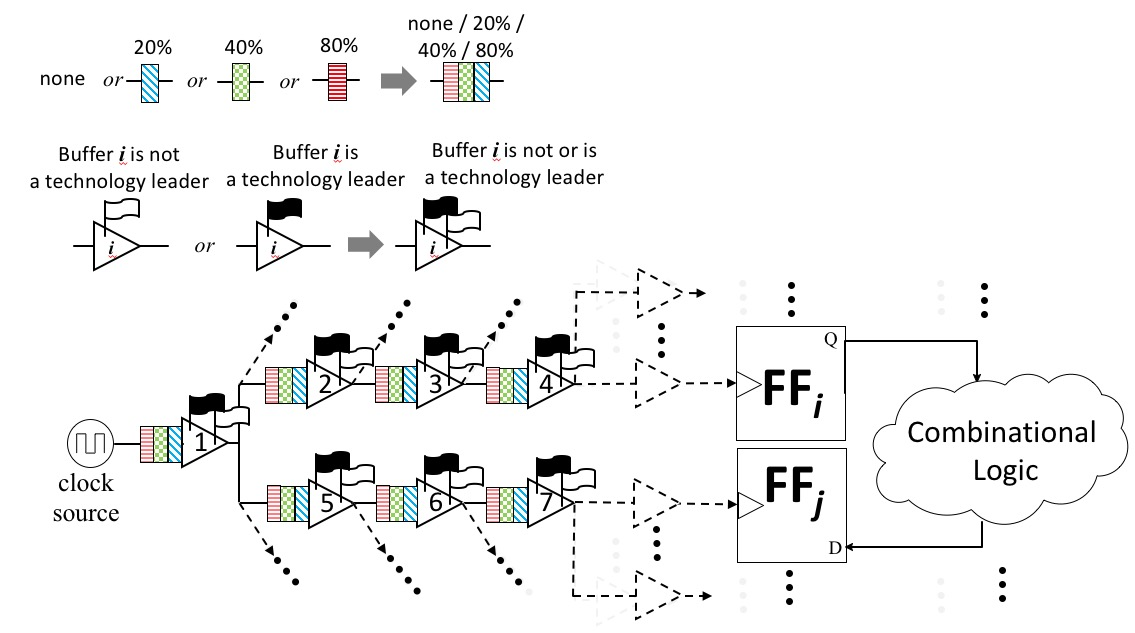
\includegraphics[width=1\columnwidth]{All_types_of_DCCs_and_leaders.png} %IEEE
	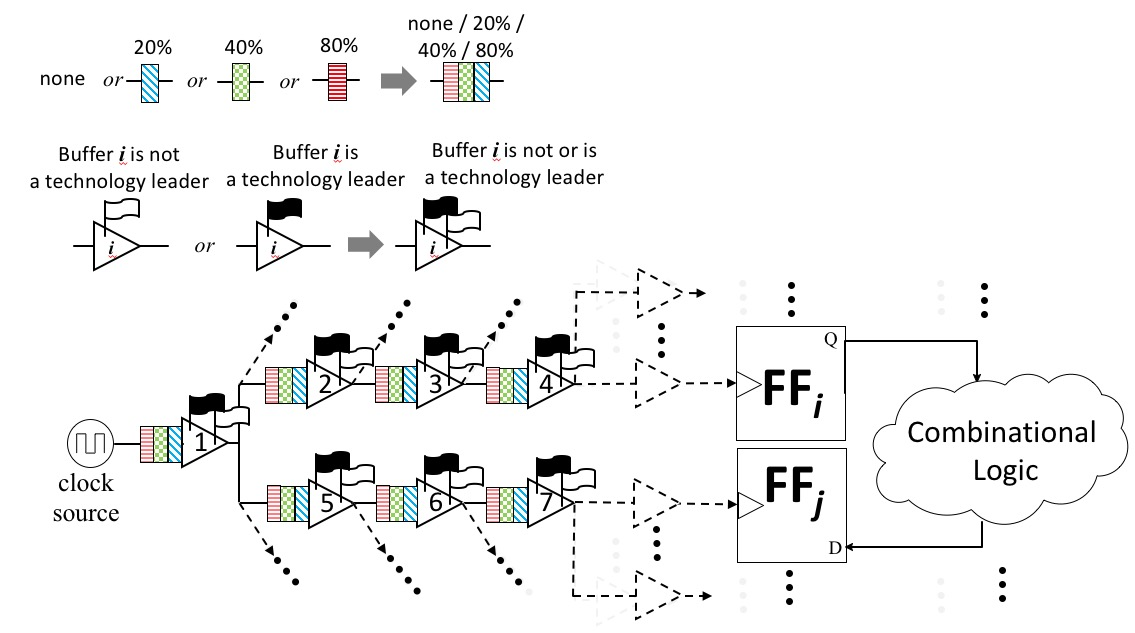
\includegraphics[width=0.8\columnwidth]{All_types_of_DCCs_and_leaders.png} %ACM
	\caption{Generalized DCC insertion and high-$V_{th}$ buffer leader selection, for a target pair of flip-flops}
	\label{fig:leadertype}
\end{figure}
\end{comment}
\begin{figure}[t!]
    \centering
    %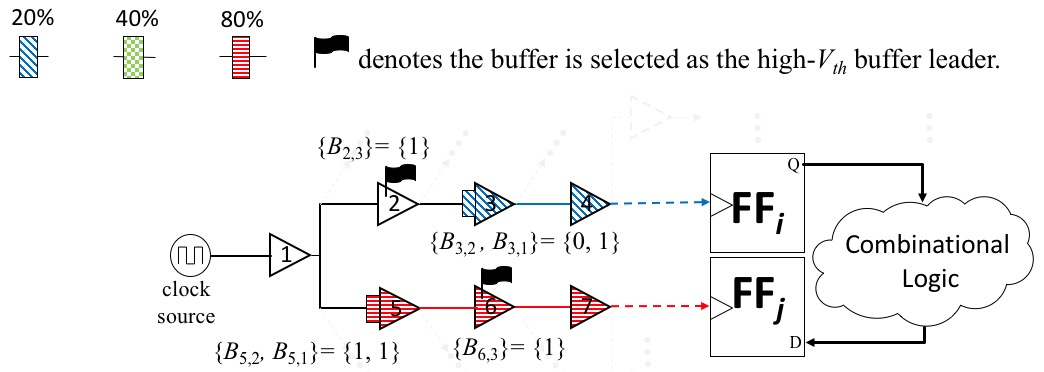
\includegraphics[width=1.0\columnwidth]{2DCC_2Leader.png} %IEEE
    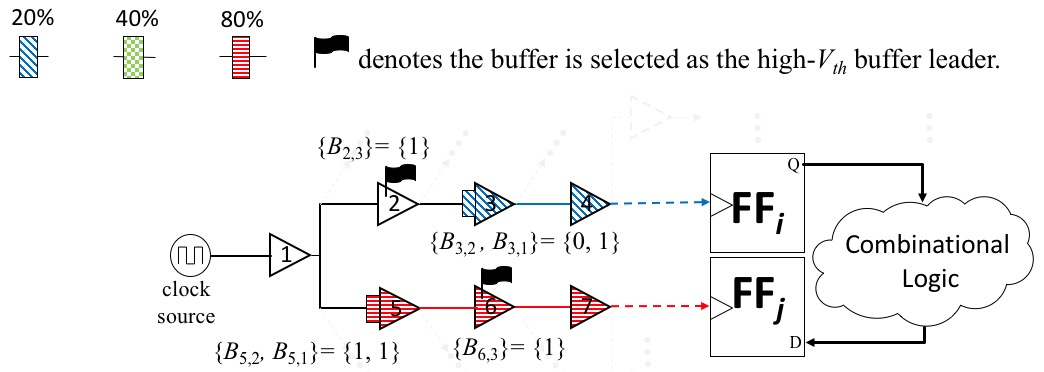
\includegraphics[width=0.71\columnwidth]{2DCC_2Leader.png} %ACM
    \caption{Example of DCC insertion and high-$V_{th}$ buffer leader selection}
    \label{fig:2dcc2leader}
\end{figure}

%Figure~\ref{fig:leadertype} shows a generalized example of DCC insertion and leader selection. It is worth reminding that, because of DCC constraints, the possibility count of DCC deployments has been dropped from 16,384 to 103. However, for each DCC deployment, there are still up to 128 ($2^7$) possibilities of leader selections, for this pair of flip-flops. Hence, we set up the following constraints on the selections of high-$V_{th}$ buffer leaders:

When two clock buffers along a single clock path are selected as leaders, the leader selection is meaningless, so that the following constraints are considered. In this way, the SAT solver will not output the corresponding leader selection in the result if the CNF is satisfiable.
%In order to suppress the occurrence of fragmentary high-$V_{th}$ assignment for clock buffers, the following constraints are considered, such that the SAT solver will not output the corresponding $V_{th}$ assignment in the result if the CNF is satisfiable.

\noindent \textbf{\uline{Leader constraints: At most one buffer along a single clock path is selected as high-$V_{th}$ buffer leader.}}

The constraints are analogous to the aforementioned DCC constraints. The corresponding clauses can be generated in a similar manner, but are not shown in the paper for brevity. In the example, the 12 clauses associated with leader constraints will be generated, in such a way that, the possibility count of leader selections is 17. Subsequently, the remaining 17 possibilities are considered in the timing constraints, introduced in the next subsection.

%------------------ Timing Constraints ()
\subsection{Timing Constraints Considering DCC Deployment and High-$V_{th}$ Assignment}
\label{sec:VTA:timing}
The timing constraints are analogous to the former timing constraints, while here we more consider the influence of high-$V_{th}$ buffer leader on clock latency. It is worth reminding that, the former timing constraints are divided into 3 classes according to the used DCC count. Because we simultaneously consider the DCC deployment and leader selection in the existing clock network, each of the former 3 classes is further divided into 3 subclasses, in terms of the leader count (0, 1 and 2). Therefore, the timing constraints are divided into 9 ($3 \times 3$) subclasses, according to the used DCC count and leader count.

For simplicity, we make an illustrative example from one of the 9 subclasses: 2 used DCCs and 2 high-$V_{th}$ buffer leaders in the clock network associated aging-critical paths in Figure~\ref{fig:2dcc2leader}, where 20\% and 80\% DCC are inserted at the inputs of buffers 3 and 5, respectively, and buffers 2 and 6 are selected as high-$V_{th}$ buffer leaders, implying that the $V_{th}$ of buffer set \{2, 3, 4\} and buffer set \{6, 7\} are assigned to high $V_{th}$ because of the leader buffer 2, 6, respectively. In the case, if it causes a timing violation along the aging-critical path, the Boolean representation of the DCC deployment and leader selection,
{\fontsize{9}{10}
\begin{gather*}
\left(\{B_{1,3}, B_{1,2}, B_{1,1}\} \equiv \{0, 0, 0\} \right) \land \left( \{B_{2,3}, B_{2,2}, B_{2,1}\} \equiv \{1, 0, 0\} \right) \land \left(\{B_{3,3}, B_{3,2}, B_{3,1}\} \equiv \{0, 0, 1\} \right) \\ 
\land \left( \{B_{4,3}, B_{4,2}, B_{4,1}\} \equiv \{0, 0, 0\} \right) \land \left(\{B_{5,3}, B_{5,2}, B_{5,1}\} \equiv \{0, 1, 1\} \right) \land \left( \{B_{6,3}, B_{6,2}, B_{6,1}\} \equiv \{1, 0, 0\} \right)\\
\land \left( \{B_{7,3}, B_{7,2}, B_{7,1}\} \equiv \{0, 0, 0\} \right),
\end{gather*}}equivalent to the following CNF clause:
{\fontsize{9}{10}
\begin{gather*}
(B_{1,3} \lor B_{1,2} \lor B_{1,1} \lor \neg B_{2,3} \lor B_{2,2} \lor B_{2,1}  \lor B_{3,3} \lor B_{3,2} \lor \neg B_{3,1} \lor B_{4,3} \lor B_{4,2} \\
\lor B_{4,1} \lor B_{5,3} \lor \neg B_{5,2} \lor \neg B_{5,1} \lor \neg  B_{6,3} \lor B_{6,2} \lor B_{6,1} \lor B_{7,3} \lor B_{7,2} \lor B_{7,1} )
\end{gather*}}should be generated such that the solver will not output the corresponding DCC deployment and leader selection in the result if the CNF is satisfiable. In this case, a total of 1 CNF clause is generated.

Note that, given the DCC deployment, if the leader count is 2, there exist 9 ($3 \times 3$) possibilities of leader selection (one among buffers $\{2, 3, 4\}$, the other one among buffers $\{5, 6, 7\}$).
If the leader count is 1/0, there exist 7/1 possibilities of leader selections. Hence, there totally exist 17 ($9+7+1$) possibilities of leader selections, for each DCC deployment.



